\subsubsection{UC 13 - Eliminare un evento} \label{sec:UC13}
    \begin{itemize}
        \item \textbf{Attore principale}: MUA;
        \item \textbf{Descrizione}: il MUA elimina un evento dal sistema;
        \item \textbf{Precondizioni}: il MUA sta usando la funzionalità di eliminazione di un oggetto;
        \item \textbf{Postcondizioni}: il sistema elimina l'evento con l'identificativo fornito dal MUA;
        \item \textbf{Scenario principale}:
            \begin{enumerate}
                \item il MUA invia i dettagli dell'evento da eliminare al sistema (\hyperref[sec:UC13.1]{UC 13.1});
                \item il sistema elimina l'evento;
            \end{enumerate}
        \item \textbf{Inclusioni}: nessuna;
        \item \textbf{Generalizzazioni}: nessuna;
        \item \textbf{Estensioni}: nessuna.
    \end{itemize}

\begin{figure}[h]
    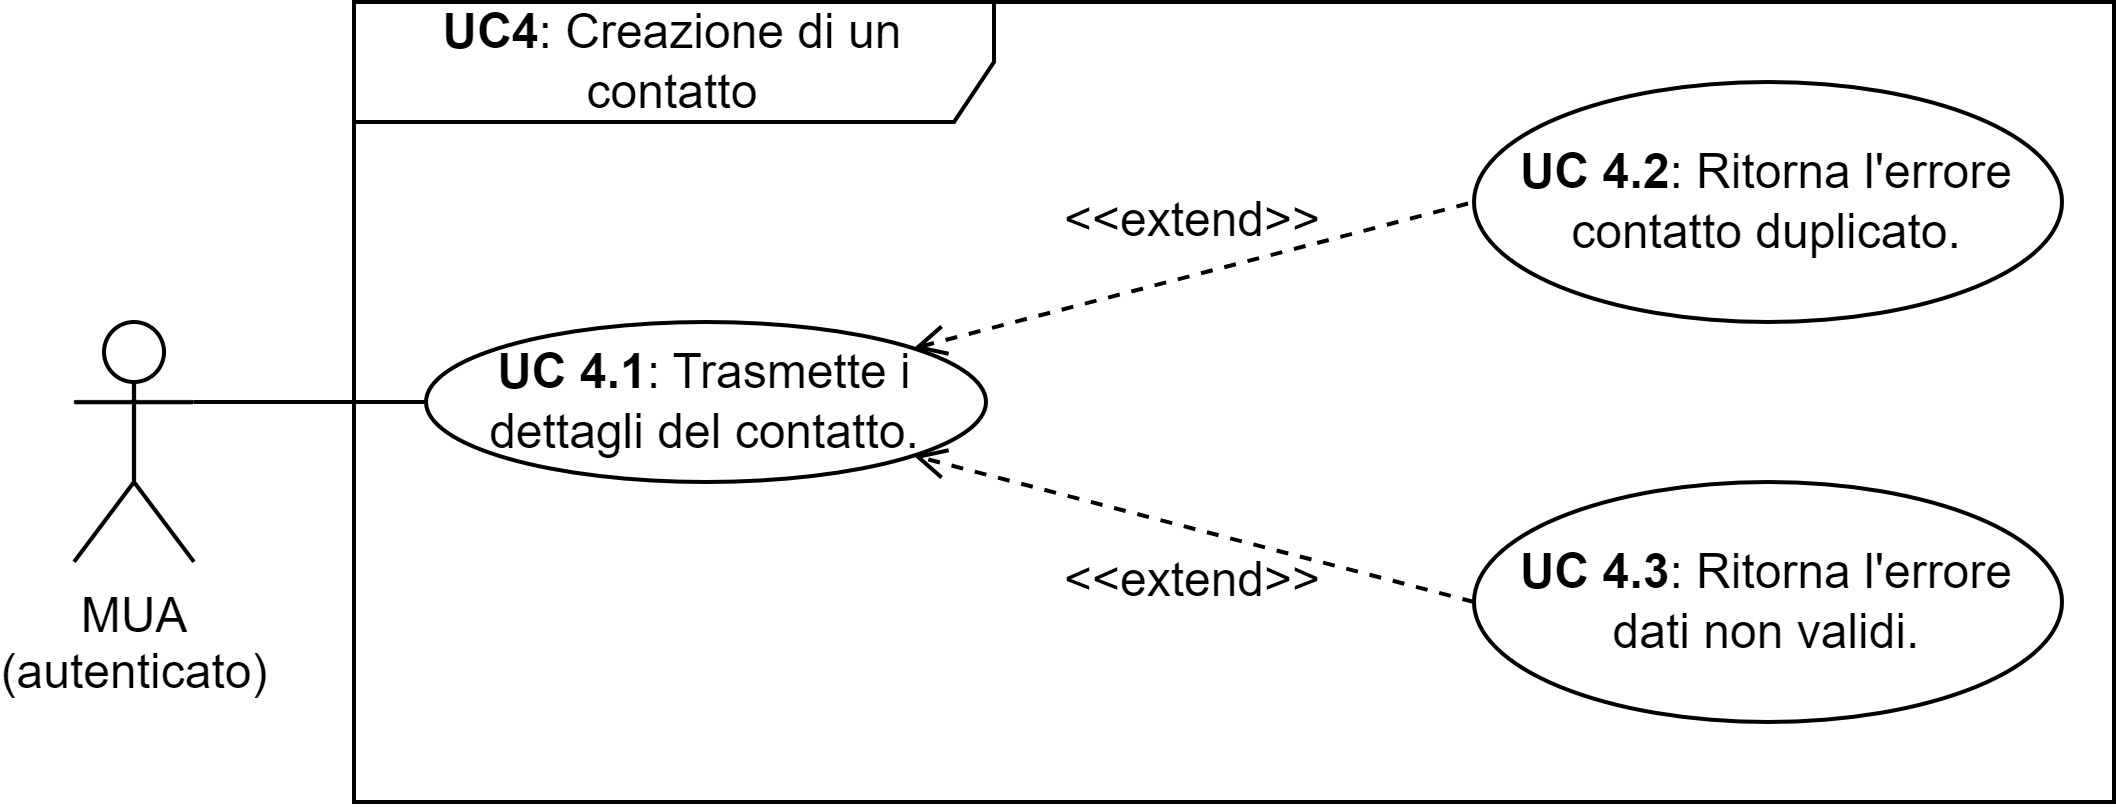
\includegraphics[width=0.85\textwidth]{sections/uc_imgs/UC04.X.png}
    \centering
    \caption{Diagramma sotto-casi UC 13.}
\end{figure}

\subsubsection{UC 13.1 - Trasmette i dettagli dell'evento} \label{sec:UC13.1}
    \begin{figure}[h]
        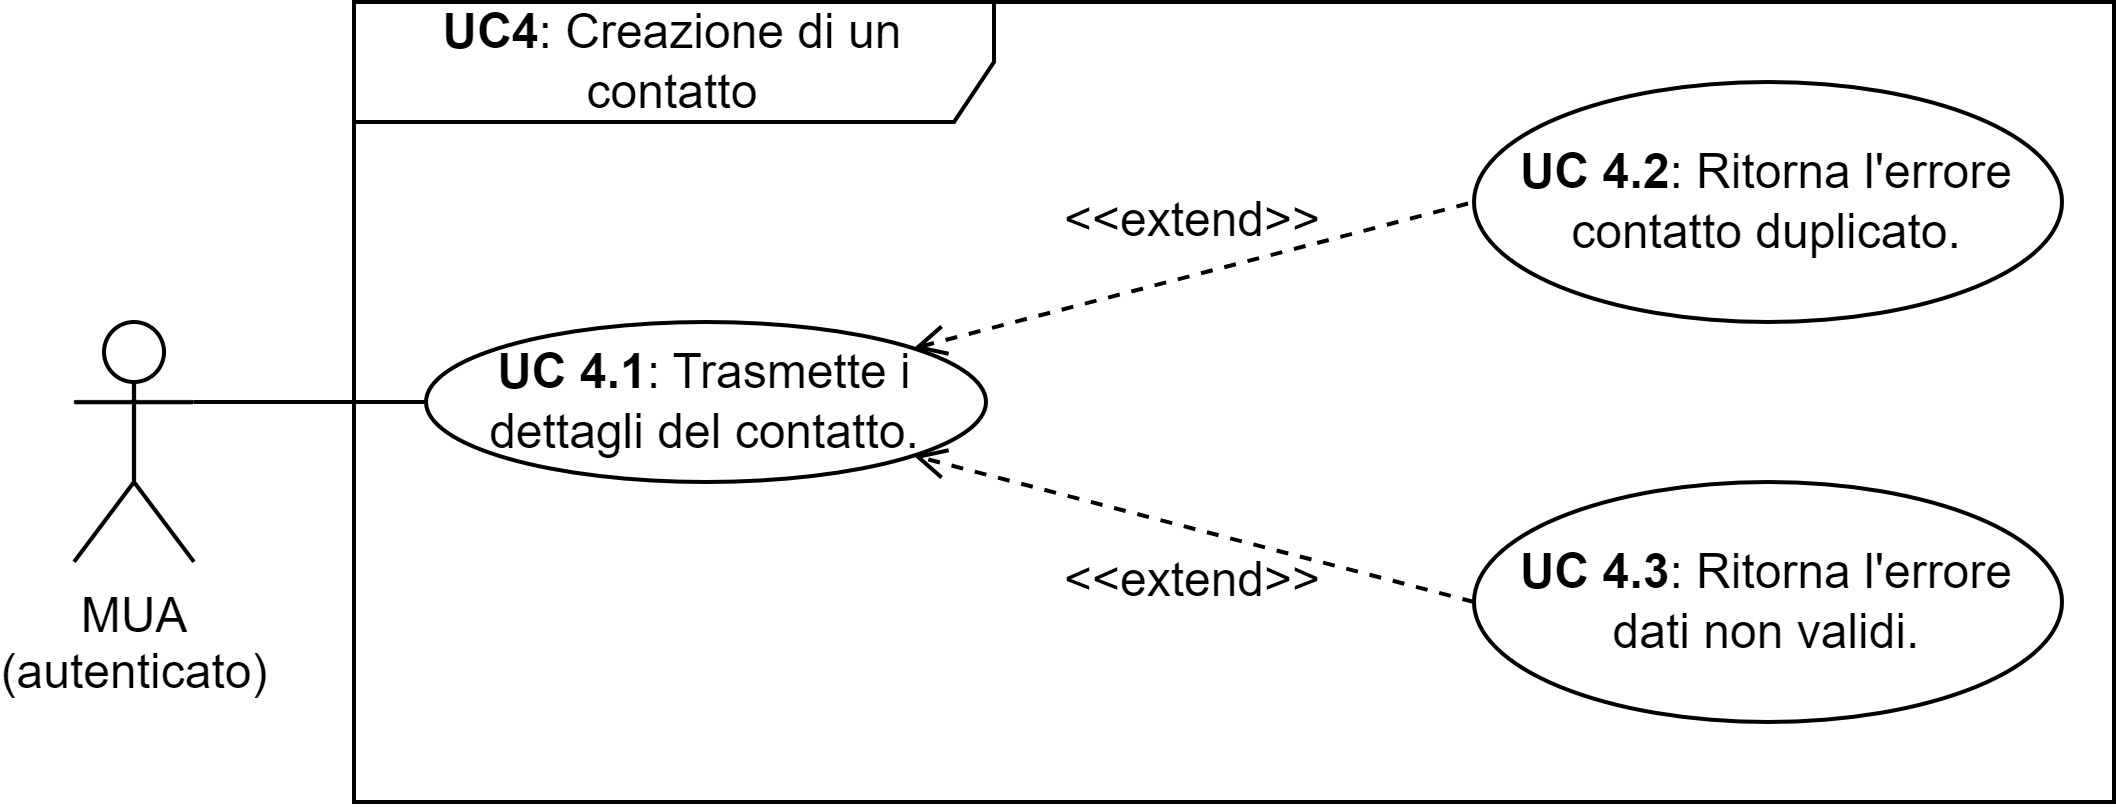
\includegraphics[width=0.85\textwidth]{sections/uc_imgs/UC04.X.png}
        \centering
        \caption{Diagramma UC 13.1.}
    \end{figure}
    \begin{itemize}
        \item \textbf{Attore principale}: MUA;
        \item \textbf{Descrizione}: il MUA invia le informazioni dell'evento da eliminare al sistema;
        \item \textbf{Precondizioni}: il MUA sta usando la funzionalità di eliminazione di un evento;
        \item \textbf{Postcondizioni}: il sistema elimina l'evento identificato dalle informazioni fornite dal MUA;
        \item \textbf{Scenario principale}:
            \begin{enumerate}
                \item il MUA invia l'identificativo dell'evento al sistema;
            \end{enumerate}
        \item \textbf{Inclusioni}: nessuna;
        \item \textbf{Generalizzazioni}: nessuna;
        \item \textbf{Estensioni}:
            \begin{enumerate}[label=\alph*.]
                \item il sistema non riesce a eliminare l'evento perché non è stato trovato:
                \begin{enumerate}[label=\arabic*.]
                    \item il sistema ritorna un errore al MUA di identificativo non valido (\hyperref[sec:UC11.2]{UC 11.2}).
                \end{enumerate}
            \end{enumerate}
    \end{itemize}


\subsubsection{UC 13.2 - Ricezione errore identificativo evento non valido} \label{sec:UC11.2}
    \begin{itemize}
        \item \textbf{Attore principale}: MUA;
        \item \textbf{Descrizione}: il sistema non riesce a eliminare l'evento perché l'identificativo evento non è stato trovato;
        \item \textbf{Precondizioni}: il MUA sta usando la funzionalità d'invio dei dettagli al sistema di un evento;
        \item \textbf{Postcondizioni}: il sistema non elimina l'evento, il MUA è stato notificato dell'errore;
        \item \textbf{Scenario principale}:
            \begin{enumerate}
                \item il sistema non trova l'evento con l'identificativo fornito dal MUA;
                \item il sistema non elimina l'evento e notifica il MUA dell'errore;
            \end{enumerate}
        \item \textbf{Inclusioni}: nessuna;
        \item \textbf{Generalizzazioni}: nessuna;
        \item \textbf{Estensioni}: nessuna.
    \end{itemize}
